\documentclass{article}
\usepackage{amsmath}
\usepackage{graphicx} % Add this line
\usepackage{xcolor}
\pagecolor{black}
\color{white}


\definecolor{lightpurple}{rgb}{0.85, 0.85, 1} % Light purple background color
\definecolor{white}{rgb}{1, 1, 1} % White text color

%\pagecolor{lightpurple}
%\color{black}

\title{Rugsafe: A Multichain Vault Protocol for Defending Against Rug Pulls}
\author{info@rugsafe.org}
\date{v0.0.1 September 1, 2024}

\begin{document}

\maketitle


\begin{abstract}
Rugsafe introduces a comprehensive protocol aimed at mitigating the risks of rug pulls in the cryptocurrency ecosystem. By utilizing cryptographic security measures and economic incentives, the protocol provides a secure multichain system for recovering assets and transforming rugged tokens into opportunities and rewards. Foundational to Rugsafe are specialized vaults where rugged tokens can be securely deposited, and anticoin tokens are issued as receipts. Users can utilize these anticoins within the ecosystem or choose to burn them, further securing the protocol and earning additional rewards. The supply of the native Rugsafe token is dynamically adjusted based on the volume, value, and activity of rugged tokens, ensuring stability and resilience. By depositing rugged tokens into a vault on several chains, and by burning anticoins, users receive incentives on the RugSafe chain. This protocol's vaults are designed to work in heterogenous blockchain ecosystems, offering a practical and effective solution to one of the most significant challenges in the cryptocurrency market. 
\end{abstract}




%\clearpage

\tableofcontents

%\twocolumn





\section{Overview}

The Rugsafe protocol enables users who hold rugged tokens, denoted as $C_r$, to deposit these tokens into a specialized vault $V_c$ and receive anticoin tokens, $C_a$,  which serve as receipts, \(\mathcal{R} \). The supply of Rugsafe's native token, $R$, is regulated based on the total value of rugged tokens in existence.

%%%%%%%%%%%%%%%%%%%%%%




\section{Definition of a Rug Pull}

A rug pull is a deceptive practice in the cryptocurrency and decentralized finance (DeFi) space, where the creators of a token, referred to as the "rug token," exploit the trust of users to siphon off liquidity and leave the victims holding worthless tokens.

\subsection{Mechanism of a Rug Pull}

1. \textbf{Creation of the Rug Token}: The token creator mints a large supply of a new token, the "rug token." The creator initially provides liquidity by pairing this rug token with another, more liquid token (e.g., ETH, USDC) and deposits both into a liquidity pool.

2. \textbf{Attracting Liquidity}: As users begin to deposit their liquid tokens into the liquidity pool, believing in the legitimacy of the rug token, the pool's liquidity increases. Users typically deposit into the pool to earn trading fees or staking rewards.

3. \textbf{Exploitation}: The token creator, who retains a significant portion of the rug token supply, waits until sufficient liquidity has been added by users. The creator then uses their large supply of rug tokens to swap out all the liquid tokens from the pool.

\[
\text{Swap} = \text{Rug Token (Large Supply)} \rightarrow \text{Liquid Token (Full Withdrawal)}
\]

4. \textbf{Outcome for Victims}: After the swap, the liquidity pool is drained of its valuable liquid tokens, leaving the victims holding a large number of rug tokens that are now worthless. The victims are left with an illiquid and devalued asset, while the creator absconds with the liquid tokens.

\[
\text{Victim's Holding} = \text{Rug Token (Now Worthless)}
\]

\subsection{Impact and Prevention}

The practice of rug pulling is highly damaging to the victims, as it results in the loss of their liquid tokens in exchange for a worthless asset. The Rugsafe protocol is designed to prevent such scenarios by introducing mechanisms that ensure tokens minted on the Rugsafe chain are rugproof by default.

Through mechanisms like bonding, claim processes, and community-driven challenge periods, the Rugsafe protocol provides a protocol to protect users from rug pulls. By requiring issuers to post a bond at token issuance and allowing the community to challenge suspected rug pulls, the protocol empowers users to take proactive steps in safeguarding their investments.

By defining and understanding the mechanics of a rug pull, the importance of the Rugsafe protocol's protective measures becomes clear. The protocol not only mitigates the risk of rug pulls but also creates a safer environment for the development and trading of new tokens within the ecosystem.





%%%%%%%%%%%%%%%%%%%%%%%%%%%%%%%%%%%%







\subsection{Vault Creation and Anticoin Issuance}
When a vault $V_c$ is created for a rugged token $C_r$, users can deposit $C_r$ into this vault. Upon deposit, the protocol mints an equal amount of $C_a$ tokens, which are credited to the user's balance. These $C_a$ tokens serve as a new, clean fungible token for the rugged victim, issued 1:1 with the underlying rugged token.

\begin{equation}
C_a = C_r
\end{equation}

In addition to the 1:1 $C_a$ tokens, the user may also receive a receipt, \(\mathcal{R} \) , in the form of a non-fungible token (NFT) or a refungible token (RFT). The 1:1 $C_a$ token acts as a standard fungible token, fully transferable and tradable. However, the receipt could also be issued as an NFT, representing a unique claim on the deposited rugged tokens. Alternatively, the receipt can be an RFT, where an NFT representing the deposit is held by a contract. The contract then distributes shares of the NFT by issuing a fungible token that serves as representative shares of the underlying NFT.

The type of asset used as the receipt, whether fungible, non-fungible, or refungible, is parameterized at the time of vault creation, with the relationship expressed as:

\[
\mathcal{R} = f(C_r, \tau)
\]

where $\text{type}$ determines whether the receipt is a fungible token, an NFT, or an RFT. This provides flexibility depending on the specific use case or preferences of the depositor. The vaults are held in a central vault registry, ensuring that all interactions with rugged tokens are tracked and managed within the system. Regardless of the type of receipt issued, depositors always receive the 1:1 $C_a$ tokens as a clean representation of their original rugged tokens.


%%%%%%%%%%%%%%%%%%%%%%%%%%%%%






\subsection{Withdrawal Penalty Mechanism}
If a user decides to withdraw their original rugged tokens $C_r$ by depositing back their $C_a$, a penalty is incurred. A portion of the $C_a$ tokens are deducted from the user's balance, and these penalized tokens are distributed among the remaining $C_a$ holders.

\begin{equation}
C_{r,w} = C_{r,d} - P(C_a)
\end{equation}

Where $P(C_a)$ represents the penalty, which scales according to the amount of $C_r$ originally deposited, \(d\). The penalty mechanism incentivizes holding $C_a$ longer, as the remaining holders benefit from these penalties.








%%%%%%%%%%%%%%%%%%%%%%%%%%%%








\subsection{Supply Regulation Mechanism}
The protocol regulates the supply of the native Rugsafe token $R$ based on the total value of all rugged tokens $C_r$ in existence. The supply of the Rugsafe token is inversely related to the sum of the values of these rugged tokens, adjusted logarithmically:

\begin{equation}
R_\text{supply}  \propto \frac{1}{\log\left(\sum C_r\right)}
\end{equation}

This mechanism ensures that as more tokens are rugged, the supply of $R$ becomes increasingly scarce, potentially enhancing its value and stability within the ecosystem.

\begin{figure}[h]
\centering
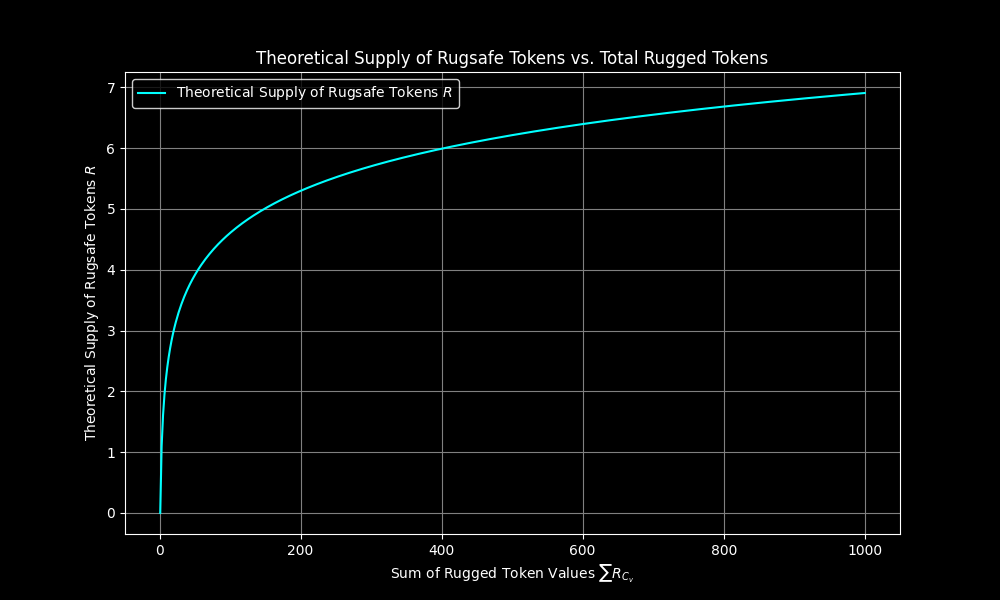
\includegraphics[width=\textwidth]{images/5.png}
\caption{The logarithmic relationship between the theoretical supply of Rugsafe tokens $R$ and the sum of rugged token values $\sum C_r$. This relationship underscores how the supply of $R$ is regulated based on the value of rugged tokens in existence, ensuring stability and scarcity.}
\label{fig:minted_anticoins}
\end{figure}

In addition to this scarcity mechanism, the native chain introduces emissions of Rugsafe tokens $R$ per block produced, as it operates on the Cosmos SDK framework. This implies that the total supply of $R$ is influenced by two opposing forces: the burning of tokens $R_\beta$ and the minting of new tokens $R_\texttt{mint}$ through block emissions.

The rate of token burning is governed by the inverse relationship with the total value of rugged tokens $C_r$ in existence:

\[
R_{\beta} \propto \frac{1}{\log\left(\sum R_{C_v}\right)}
\]

Simultaneously, the protocol continuously mints new tokens at a rate proportional to the number of blocks produced:

\[
R_{\texttt{mint}} = \epsilon \times b
\]

where $\text{emission\_rate}$ is a parameter that determines the number of Rugsafe tokens emitted per block.

The net change in the supply of Rugsafe tokens $R_\text{net}$ over time is the difference between the tokens minted and burned:

\[
R_{\text{net}} = R_{\epsilon} - R_{\beta}
\]

Both the burn rate $R_{\beta}$ and the emission rate per block $R_\epsilon$ are parameterized and can be adjusted through community governance:

\[
R_\beta = f\left(\frac{1}{\log\left(\sum R_{C_v}\right)}, \beta_{\texttt{burn}}\right)
\]


and to calculate the amount minted, we can take the emission rate per block, multiplied by the amount of blocks considered,

\[
R_{\beta} = g(\epsilon, \text{blocks})
\]

This flexibility allows the community to respond to changing market conditions and fine-tune the protocol to achieve the desired balance between token scarcity and availability. By giving the community control over these parameters, the protocol ensures that it can adapt over time, maintaining the health and stability of the Rugsafe ecosystem.




%%%%%%%%%%%%%%%%%%%%%%%%%%%%%%%







\subsection{Anticoin Role and Market Interaction}
At the time of vault creation, the protocol mints $C_a$ tokens in a 1:1 ratio with the deposited rugged tokens $C_r$. These $C_a$ tokens serve as a clean, fungible representation of the rugged tokens, providing users with a new asset that can be freely traded or held. The value of $C_a$ tokens is determined entirely by market forces, \(m_f\), allowing the broader ecosystem to establish their worth relative to other assets.

The $C_a$ tokens function purely as receipts for the deposited rugged tokens and do not undergo any price adjustments or pegging mechanisms. This approach ensures that the protocol remains simple and transparent, with the market dictating the value of $C_a$ based on supply and demand dynamics.




%%%%%%%%%%%%%%%%%%%%%%%%%%%%%%%
%%%%%%%%%%%%%%%%%%%%%%%
%%%%%%%%%%%%%%%%%




\subsection{User Interaction and Ecosystem Signaling}
When users deposit rugged tokens $C_r$ into a vault $V_c$, they receive $C_a$ tokens as a direct and clean representation of their deposited rugged tokens. The relationship between the deposited tokens and the minted $C_a$ tokens is given by:

\[
C_a = C_r
\]

These $C_a$ tokens function as receipts, representing the ownership and claim on the underlying rugged tokens. The $C_a$ tokens are fungible and can be freely used within the ecosystem, whether for trading, holding, or as collateral in other DeFi applications. The presence of $C_a$ tokens within the market serves as a signal that the user has deposited rugged tokens into the protocol, effectively transforming $C_r$ into a new, market-driven asset.

The market value of $C_a$ tokens is influenced by several factors, including:

1. \textbf{Market Supply and Demand}: The value of $C_a$ tokens, $P_{C_a}$, is determined by the market, where supply and demand dynamics play a crucial role:

\[
P_{C_a} = f(S_{C_a}, D_{C_a})
\]

As the demand for $C_a$ tokens increases relative to their supply, the market value $P_{C_a}$ will rise, and vice versa.

2. \textbf{Underlying Value of Rugged Tokens}: The value of $C_a$ tokens is also indirectly linked to the perceived value of the underlying rugged tokens $C_r$. If the market expects that the rugged tokens $C_r$ might regain value in the future, the value of $C_a$ could increase accordingly:

\[
P_{C_a} \propto E(P_{C_r})
\]

where $E(P_{C_r})$ is the expected future value of the rugged tokens.

3. \textbf{Liquidity and Utility}: The utility of $C_a$ tokens within the ecosystem—such as their use as collateral, in trading pairs, or in yield farming—contributes to their liquidity and market value. The more integrated and useful $C_a$ tokens are within the DeFi space, the higher their market value:

\[
P_{C_a} = g(U_{C_a}, L_{C_a})
\]

The protocol does not enforce any actions related to burning or altering the supply of $C_a$ tokens. Instead, the focus is on providing a straightforward receipt mechanism that empowers users to manage their assets independently within the ecosystem. This means that $C_a$ tokens remain purely market-driven assets, with their value being dictated by market conditions and the broader DeFi ecosystem. 

Users may choose to hold $C_a$ tokens, anticipating a rise in value due to market demand or the recovery of the underlying rugged tokens. Alternatively, they might trade or leverage $C_a$ in other DeFi applications, thereby influencing its liquidity and market presence.

This design choice simplifies the user experience while maintaining the integrity and transparency of the protocol. The absence of enforced mechanisms like burning or minting ensures that the value of $C_a$ tokens is wholly determined by the market, reflecting real-time supply and demand conditions within the ecosystem.





%%%%%%%%%%%%%%%%%%%%%%%




\subsection{Opportunities for New Ecosystems}
The Rugsafe protocol's structure introduces significant opportunities for developers and communities associated with rugged tokens $C_r$. Each rugged token $C_r$ represents an ecosystem that anticipated a specific offering or vision to materialize within the market. The issuance of $C_a$ tokens as a clean, fungible representation of $C_r$ provides these communities with a renewed opportunity to realize their original goals.

By depositing rugged tokens $C_r$ into a vault $V_c$, the protocol mints $C_a$ tokens in a 1:1 ratio:

\[
C_a = C_r
\]

These $C_a$ tokens, backed by provable deposits of the original underlying rugged tokens, allow communities to reintroduce their vision to the market under new terms. The $C_a$ tokens can be traded, utilized as collateral, or integrated into new decentralized finance (DeFi) applications, thereby reviving the ecosystem that was initially disrupted.

The presence of $C_a$ tokens in the market not only provides a second chance for these communities but also creates new financial products and services tailored to support the specific needs of rug pull victims. Developers can leverage this mechanism to build applications that cater to these communities, effectively transforming $C_r$ from a symbol of loss into a foundation for new economic activity.

Quantifying the impact, if $N$ is the total number of rugged tokens and $M$ represents the market value of each token, the introduction of $C_a$ creates a new market potential:

\[
\text{Market Potential} = \sum_{i=1}^{N} M_i \cdot C_{a,i}
\]

This market potential signifies the total value that can be recaptured or reintroduced into the ecosystem through $C_a$ tokens, providing a substantial incentive for developers and communities to participate in the Rugsafe protocol. The resulting ecosystem could not only restore lost value but also innovate new financial instruments and services, revitalizing the original vision of the rugged projects.





%%%%%%%%%%%%%%%%%%%%%%%%%%%




\subsection{User Commitment and Signal to the Ecosystem}

Depositing $C_r$ into a vault $V_c$ and receiving $C_a$ tokens signals the user's belief that $C_r$ is a rugged token. This action converts the rugged tokens into a new, clean representation within the ecosystem. To demonstrate a stronger commitment to the protocol, users can choose to burn their $C_a$ tokens, effectively removing them from circulation. This act of burning is a significant signal within the ecosystem.

The burning process can be represented as:

\[
\text{Signal} = \texttt{Burn}(C_a)
\]

Mathematically, the burning mechanism reduces the circulating supply of $C_a$ tokens, which can be expressed as:

\[
C_a' = C_a - B_{C_a}
\]

where \(C_a'\) is the circulating supply of $C_a$ after the burn, and \(B_{C_a}\) is the quantity of $C_a$ tokens burned.

This reduction in supply impacts the overall market dynamics and is reflected in the inverse relationship between the value of the Rugsafe token $R$ and the volume of rugged tokens $C_r$:

\[
R_\text{supply}  \propto \frac{1}{\log\left(\sum C_r \right)}
\]

The act of burning $C_a$ tokens strengthens this relationship by increasing the scarcity of $C_a$ and consequently affecting the value of $R$. The more $C_a$ is burned, the greater the signal of commitment to the protocol, potentially leading to a stronger inverse correlation between the value of $R$ and the total rugged tokens $C_r$.

\[
\frac{\partial R}{\partial C_a} < 0
\]

This partial derivative indicates that as the circulating supply of $C_a$ decreases (through burning), the value of $R$ is expected to increase, further solidifying the protocol's stability and the commitment of its participants.

%% could be problematic



%%%%%%%%%%%%%%%%%%%%%%%%%%%%%%%%%%%






\subsection{Rugsafe Vaults as Oracles}
Rugsafe vaults act as decentralized oracles, providing reliable data on the existence and volume of rugged tokens. This oracle functionality enables the protocol to adjust the supply of $R$ accurately and in real-time, based on the real-world data collected from the vaults.



%%%%%%%%%%%%%%%%%%%%%%%%%%%%%

















%%%%%%%%%%%%%%%%%%%%%%%%





\subsection{Whale Penalty Mechanism}
To prevent large holders (whales) from gaming the system, the penalty for withdrawing rugged tokens $C_r$ scales with the amount of $C_a$ held. This mechanism is inspired by quadratic voting schemes, where the penalty increases progressively as the holder's balance of $C_a$ tokens grows, ensuring fairness and preventing manipulation. the penalty $P(C_a)$ for withdrawing rugged tokens is mathematically represented as:


\[
P(C_a) \propto \left(H_{C_a}\right)^\lambda
\]

Where $\lambda > 1$ is a scaling factor that ensures the penalty increases non-linearly with the amount of $C_a$ held.

\subsubsection{Impact on regular users vs. whales}

For regular users, who typically hold smaller amounts of $C_a$, the penalty remains relatively low, as the function’s exponent $\lambda$ ensures that the penalty grows slowly with their holdings:

\[
P_{\text{regular}}(C_a) = k \cdot \left(H_{C_a}\right)^\lambda \quad \text{with} \quad \lambda > 1 \quad \text{and} \quad H_{C_a} \text{ small}
\]

Where $k$ is a proportionality constant. for these users, the impact of the penalty is minimal, allowing them to interact with the protocol without significant costs, thus promoting fairness and inclusivity.

For whales, however, the penalty increases significantly due to their large holdings of $C_a$. as the amount of $C_a$ held by a whale increases, the penalty grows more steeply:

\[
P_{\text{whale}}(C_a) = k \cdot \left(H_{C_a}\right)^\lambda \quad \text{with} \quad \lambda > 1 \quad \text{and} \quad H_{C_a} \text{ large}
\]

This non-linear increase in penalty serves two purposes. first, it deters whales from attempting to manipulate the system by accumulating and withdrawing large amounts of $C_r$. Second, it ensures that whales, who may also be regular users of the protocol, are subject to the same rules but with penalties that reflect their larger influence on the system.

\subsubsection{Equitable system design}

\begin{figure}[h]
\centering
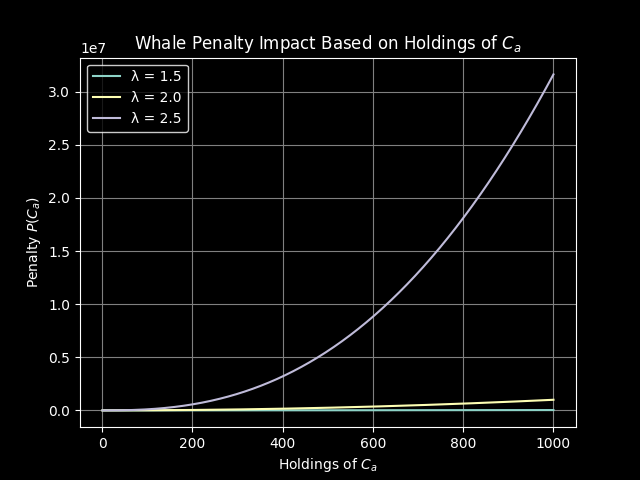
\includegraphics[width=\textwidth]{images/6.png}
\caption{the impact of the whale penalty mechanism based on varying scaling factors $\lambda$. as $\lambda$ increases, the penalty for holding larger amounts of $C_a$ grows exponentially, particularly affecting whales with significant holdings.}
\label{fig:whale_penalty}
\end{figure}


By scaling the penalty non-linearly with the amount of $C_a$ held, as in figure \ref{fig:whale_penalty}, the system remains equitable for all users, regardless of their holdings. Regular users are protected from disproportionate penalties, while whales, whose actions could have a more significant impact on the system, face penalties commensurate with their holdings. This design discourages potential manipulation by large holders and promotes a more balanced and fair ecosystem for all participants.

\subsubsection{Cumulative penalty mechanism}

\begin{figure}[h]
\centering
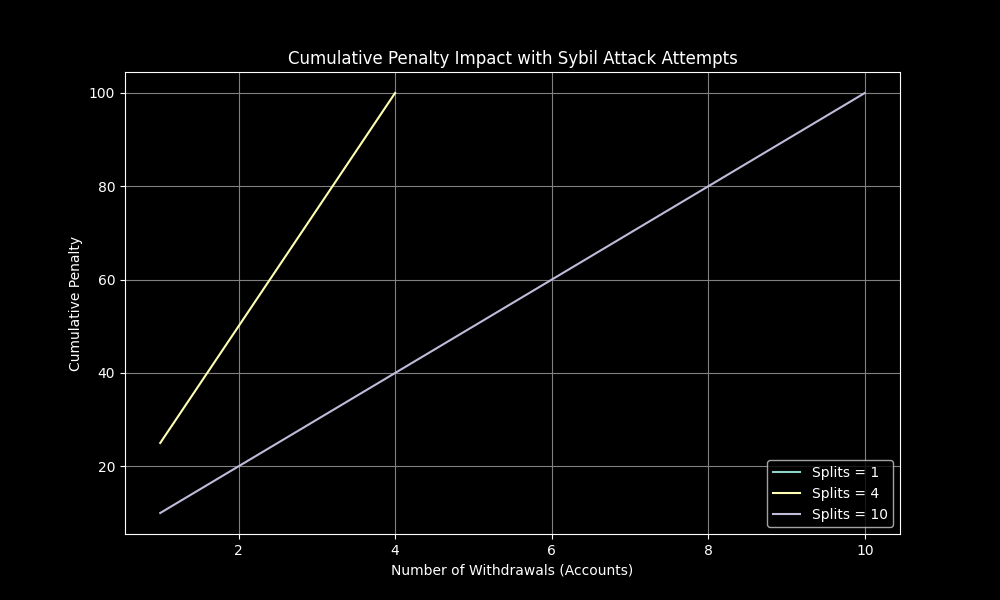
\includegraphics[width=\textwidth]{images/9.png}
\caption{the impact of the cumulative penalty mechanism on sybil attack attempts. the more accounts a whale creates to split their holdings, the higher the cumulative penalty becomes, discouraging such behavior.}
\label{fig:cumulative_penalty}
\end{figure}


To further enhance the protocol's defense against potential sybil attacks, a cumulative penalty mechanism has been introduced. This mechanism accumulates penalties progressively with each withdrawal attempt, particularly when a whale attempts to split their holdings across multiple accounts to evade higher penalties.

In this approach, the cumulative penalty is applied on a per-account basis but is aggregated across all related accounts. As illustrated in figure \ref{fig:cumulative_penalty}, the more accounts a whale creates to distribute their holdings, the more significant the overall penalty becomes. This cumulative effect discourages sybil attacks by ensuring that the total penalty incurred across all accounts exceeds what would have been paid if the whale had used a single account.

\[
P_{\text{cumulative}}(C_a) = P(C_a) \times \text{number of withdrawals}
\]

This means that while the whale may try to avoid the higher penalties by splitting their holdings across multiple accounts, the total cumulative penalty across those accounts will still be greater than the penalty they would have faced had they withdrawn the entire amount in a single transaction.

This can be seen in the plot below, where splitting across more accounts results in steeper cumulative penalties. the yellow and purple lines represent penalties for whales trying to split their holdings across 4 and 10 accounts, respectively.



%%%%%%





\subsubsection{Combining both mechanisms}

By combining the original non-linear penalty mechanism (which targets large holdings) with the cumulative penalty mechanism (which penalizes sybil attack attempts), the protocol ensures that whales are doubly disincentivized from trying to game the system. 

Whales face increasing penalties for holding large amounts of $C_a$. They also face additional cumulative penalties if they attempt to circumvent the system through sybil attacks by distributing their holdings across multiple accounts.

To formally prove that a whale attempting to split their holdings across multiple accounts incurs a higher penalty than withdrawing the entire amount in one transaction, consider the following:

\subsubsection{One-time withdrawal}

For a whale holding $H_{total}$ tokens, the penalty for a single withdrawal is:

\[
P_{\text{one-time}} = H_{total} \times \gamma
\]

Where $\gamma$ is the penalty rate (e.g., 10\%).

\subsubsection{Sybil withdrawal}

If the whale splits $H_{total}$ into $n$ accounts, the penalty for each account is given by:

\[
P_{\text{split}} = \left(\frac{H_{total}}{n}\right) \times \gamma
\]

The cumulative penalty is the sum of penalties across all $n$ accounts:

\[
P_{\text{cumulative}} = \sum_{i=1}^{n} \left( \frac{H_{total}}{n} \times \left( \gamma + \Delta \gamma \times i \right) \right)
\]

Where $\Delta \gamma$ is the incremental penalty applied to each subsequent withdrawal (i.e., cumulative penalty mechanism).

Simplifying this expression:

\[
P_{\text{cumulative}} = H_{total} \times \gamma + \frac{H_{total} \times \Delta \gamma \times n}{2}
\]

This expression shows that the cumulative penalty grows with both the number of splits $n$ and the incremental penalty $\Delta \gamma$, resulting in a total penalty that is higher than the one-time withdrawal penalty:

\[
P_{\text{cumulative}} > P_{\text{one-time}}
\]

Therefore, attempting to game the system through sybil attacks (splitting tokens across multiple accounts) leads to a higher overall penalty, as the cumulative penalty mechanism introduces increasing costs with each additional withdrawal.

This combined system ensures the integrity of the protocol by preventing manipulative behaviors and promoting fairness for all participants.










%%%%%%%%%%%%%%%%%%%%%%%%%%%%%%%%%%%%%


\subsection{Rugsafe Token Emissions and Parameterized Rewards Mechanism}

The Rugsafe protocol introduces a mechanism that incentivizes users to deposit rugged tokens $C_r$ into vaults $V_c$ by providing rewards in the form of Rugsafe tokens $R$. These vaults, serving as oracles, verify the deposits of specific rugged tokens and trigger emissions of Rugsafe tokens on the main chain.

In addition to receiving $C_a$, the user is rewarded with an airdrop of Rugsafe tokens $R$ on the main chain. The reward amount, $R_{\omega}$, for depositing rugged tokens is parameterized at the time of vault creation and is expressed as a function of the value of the deposit:

\[
R_{\omega} = f(C_r, \omega)
\]

where $\omega$ is a parameter set during vault creation that determines the emission rate tied to the value of the deposited tokens.

Furthermore, the protocol introduces a greater incentive for users who choose to burn their $C_a$ tokens, thereby signaling that they do not intend to redeem their underlying rugged tokens. The reward amount for burning, $R_{\texttt{burn}}$, is also parameterized at vault creation and is given by:

\[
R_{\texttt{burn}} = g(C_a, \theta) \quad \text{with} \quad g(C_a, \theta) > f(C_r, \omega)
\]

where $\theta$ is a parameter that sets a higher emission rate for burning $C_a$, indicating a permanent withdrawal of the rugged tokens from circulation.

Both the deposit and burn reward rates are flexible and can be tailored to the specific needs of the vault or community at the time of creation. This parameterization allows for customization of the incentives to align with the objectives of the protocol and the specific rugged token ecosystem.

This mechanism ensures that users are rewarded for contributing to the stability and security of the Rugsafe ecosystem. By depositing $C_r$ into vaults and potentially burning $C_a$, users receive Rugsafe tokens, fostering further participation and engagement in the protocol. The difference in reward levels between depositing and burning reflects the varying degrees of commitment to the ecosystem, with greater rewards for those who choose to fully transition away from their rugged tokens.





%%%%%%%%%%%%%%%%%%%%%%%%%%%%%%%%%%%%%%%%%








\subsection{Rugproof Mechanism}

The Rugsafe chain introduces a novel mechanism that allows users to mint new assets directly on the chain, with the assurance that these assets are rugproof by default. This mechanism is designed to protect users from potential rug pulls by leveraging a bonding system and a community-driven challenge process.

\subsubsection{Token Issuance and Bonding Mechanism}

At the time of token issuance, the issuer is required to put up a nontrivial percentage \(x\%\) of the total issued tokens as a bond:

\[
\beta_{\text{issuer}} = x\% \times T_I
\]

This bond acts as collateral, ensuring that the issuer has a stake in the integrity of the project. The bond is held in escrow and serves as a safeguard against potential rug pulls.

\subsubsection{Claim and Challenge Process}

At any point in time, any user can submit a claim against the token issuer, asserting that the project is being rugged. To submit a claim, the user must also put up a bond, \(\beta_{\text{claim}}\), as a guarantee of their claim:

\[
\beta_{\text{claim}} = y\% \times T_I
\]

where \(y\%\) is a parameter that may vary depending on the perceived risk or the specifics of the token.

Upon submitting a claim, a challenge period begins, during which other users can vote on whether the project is indeed rugging. Each vote requires a deposit, \(\delta_{\text{vote}}\), which can be chosen by the voter, though it may be smaller than the claim bond:

\[
\delta_{\text{vote}} \geq z
\]

where \(z\) is a minimum deposit amount set by the protocol.

\subsubsection{Outcome of the Challenge Period}

At the conclusion of the challenge period, the following outcomes are possible:

1. \textbf{Project Found to Be Rugging}: If the project is found to be rugging, the issuer's bond is slashed by a parameterized percentage, \(\alpha\%\), and distributed among all token holders, excluding the issuer:

\[
\beta_{\text{slashed}} = \alpha\% \times \beta_{\text{issuer}}
\]

The user who successfully claimed the rug pull receives a larger portion of the slashed bond, with the remaining amount distributed among the users who supported the claim.

2. \textbf{Claim Found to Be Fraudulent}: If the claim is found to be fraudulent, the claim bond is slashed by a parameterized percentage, \(\gamma\%\), and distributed to those who voted against the claim:

\[
\beta_{\text{slashed}_{\text{claim}}} = \gamma\% \times \beta_{\text{claim}}
\]

This process discourages false claims and encourages honest participation in the challenge process.

\subsubsection{Incentives and Protection}

This mechanism incentivizes users to carefully consider their actions when minting new assets and making claims. The initial bond posted by the issuer serves as a deterrent against rug pulls, while the challenge process allows the community to actively monitor and vote on the integrity of the project. By requiring bonds for claims and votes, the protocol ensures that participants have a stake in the outcome, reducing the likelihood of frivolous claims or votes.

By implementing this mechanism, the Rugsafe chain offers a robust, community-driven solution to protect users from potential rug pulls before they occur. This not only enhances the security of the ecosystem but also empowers users to take an active role in maintaining the integrity of the projects they support.



%%%%%%%%%%%%%%%%%%%%%%%%%%%%%%%%%%%%%%%










%%%% rugproof mechanism


\section{Closing Remarks}
The prevalence of rug pulls represents one of the most pressing threats to the integrity and trust in the cryptocurrency ecosystem. Rugsafe is committed to addressing this challenge by leveraging advanced technology and innovative mechanisms to protect users from rug pulls. By providing a secure framework for asset recovery and offering tools that prevent malicious activity, Rugsafe seeks to eliminate one of the largest sources of financial loss in the industry. Rugsafe’s mission is to transform vulnerabilities into resilience, ensuring that digital assets are protected and confidence in the market is restored.

\end{document}


% things to add
% perpetuals market
% asymmetric funding rates
% anticoins inverse price with dex
% defi suite
% prediction market
% borroing and lending
